\documentclass[tikz,border=6pt]{standalone}
\usepackage{amsmath,amssymb}
\definecolor{inM}{RGB}{31,94,165}\definecolor{inC}{RGB}{214,96,33}
\tikzset{
  m/.style={circle,inner sep=0pt,minimum size=9pt,ball color=inM!85,draw=inM!60!black,line width=0.3pt},
  c/.style={circle,inner sep=0pt,minimum size=9pt,ball color=inC!90,draw=inC!60!black,line width=0.3pt},
  lab/.style={font=\small,fill=white,fill opacity=0.85,text opacity=1,inner sep=1.2pt,rounded corners=1pt},
  e/.style={line width=0.75pt,black!55},
  ec/.style={line width=1.5pt,inC!80!black}}
\begin{document}
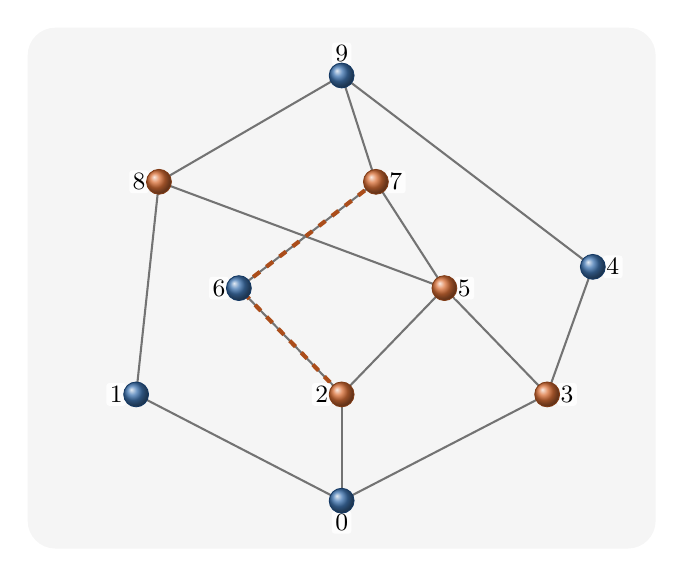
\begin{tikzpicture}[x=1.45cm,y=1.35cm]
\fill[black!4,rounded corners=10pt] (-2.75,-0.45) rectangle (2.75,4.45);
\coordinate (0) at (0,0);
\coordinate (1) at (-1.8,1); \coordinate (2) at (0,1); \coordinate (3) at (1.8,1);
\coordinate (6) at (-0.9,2); \coordinate (5) at (0.9,2); \coordinate (4) at (2.2,2.2);
\coordinate (8) at (-1.6,3); \coordinate (7) at (0.3,3);
\coordinate (9) at (0,4);
\foreach \u/\v in {0/1,0/2,0/3,1/8,2/5,2/6,3/4,3/5,4/9,5/7,5/8,6/7,7/9,8/9}
  \draw[e] (\u) -- (\v);
\draw[ec,dashed] (2) -- (6) -- (7);
\foreach \n/\p in {0/below,1/left,2/left,3/right,4/right,5/right,6/left,7/right,8/left,9/above}
  \node[lab,\p=3.5pt] at (\n) {$\n$};
\foreach \n in {0,1,4,6,9} \node[m] at (\n) {};
\foreach \n in {2,3,5,7,8} \node[c] at (\n) {};
\end{tikzpicture}
\end{document}
